\documentclass[12pt]{article}


\usepackage{amsmath}
\usepackage{amssymb}
\usepackage{graphicx}
\usepackage{geometry}
\usepackage{hyperref}

\geometry{
letterpaper,tmargin=1in,bmargin=1in,lmargin=1in,rmargin=1in
}


\begin{document}
\title{PDR: Remote Vibration Sensing\\ Team: Positive Resonance}

\author{Muneer Tatum, Jeffery Thorpe, Justin Koester, Ethan Puerto, Joe Stinson}

\date{10/10/2016}
\maketitle
\tableofcontents
\newpage
\section{Introduction}

\quad \ Sometimes the construction of a structure can cause harm to existing structures. Every time a new structure is constructed machines bring materials, place materials, and excavate raw material. Each one of these actions creates vibration in the ground that, if a certain frequency is reached, can disrupt surrounding structures. For instance, a pile driver repeatedly slamming cement poles into the ground may produce a vibration whose frequency can causes the ceramic moldings on a important building near by to crack and fall from the ceiling.\\

Since the 1930's these seismic phenomenons have been measured and studied, and various types of vibration sensors have been invented. There are sensors that can be left on site over prolonged periods of time, where a worker can obtain readings directly from the sensor as needed.  Other available sensors can send a signal when hazardous vibrations are sensed through blue tooth, and flash a warning light to alert on-site crew members.  One sensor, the Vibra-Tech Multi-Seis Plus can do many of these things, but is a costly option.  \\

One feature that many of these devices do not have is connectivity to the web, and with the advancements in technology, evolving direct connectivity is the next step for sensor technology. The best sensor on the market may not be the one with all the bells and whistles such as the previously mentioned Vibra-Tech Multi-Seis Plus; the best just needs to get the most important measurements, while transmitting them to the user in a real time fashion allowing competitive edge, and reliable function.            
\newpage

\section{Client Needs}





Currently, regulations are in place to protect existing structures that include monitoring vibrations and tracking construction related seismic activity within a 500 ft radius of a construction site. The company Smart Structures is following said rules, but it is not efficient or cost effective to do so. Currently Smart Structures has an operator set up a device or devices, and then physically monitor them on a weekly basis, downloading data and making adjustments to the construction process as needed in order to protect the surrounding structures.  To reduce man hours and foot work, Smart Structures needs a remote way to gather and upload vibration data.  These devices will transmit data to a server for collection and send vibration alerts regarding frequencies that surpass the response threshold to necessary personnel.\\

In order to determine the appropriate solution, the needs must first be assessed by the client as follows:\\

\begin{enumerate}
	\item Obtaining measurements
	\begin{enumerate}
		\item Client has requested a new weatherproof system customized to be the most effective for their construction needs.
		\item Sensor should accurately measure vibrations from 2Hz-500Hz.
		\item Be consistent \& precise.
		\item Respond promptly to events.
	\end{enumerate}
	
	\item Tabulated Data
	\begin{enumerate}
		\item Should be modifiable to client needs.
		\item Represent data effectively.
		\item Be able to be acquired by multiple routes.
	\end{enumerate}
	
	\item Real time measurements
	\begin{enumerate}
		\item Best route of communication is via simultaneous cloud transmission, text message alerting, email alerting, along with visual warning from the device.
		\item Non-Alerting measurements need not be real time unless prompted.
	\end{enumerate}
	\item Connectivity
	\begin{enumerate}
		\item Device needs to connect to existing wi/fi when available.
		\item Device should be able to switch to 4G signal when wi/fi is unavailable.
	\end{enumerate}
	\item Robust sensor housing
	\begin{enumerate}
		\item Sensor system will be placed outdoors in residential areas, commercial areas, forests, etc\dots 
		\item Device must withstand all environmental conditions.
		\item Impact resistant within reason. 
	\end{enumerate}
	\item Battery life
	\begin{enumerate}
		\item Device needs to run hands free for minimum of 1 month.
		\item Device must be rechargeable.
	\end{enumerate}
	\item Methods of recharging
	\begin{enumerate}
		\item Customer preference to solar recharging capabilities.
		\item Alternate methods optional.
		\item Recharging method must also be able to weather environmental conditions.
	\end{enumerate}
\end{enumerate}


\section{Gantt Chart}

The Gantt chart is attached.
\subsection{Summary}

Our gantt chart illustrates a critical outline schedule for the conception and creation of the Vibration Sensor. The tasks on the chart are labeled with the task names and team members that are responsible for completing those tasks. The black colored bars represent main tasks, while the blue bars represent subtasks. The thinner bars located inside the thicker bars represent the progress percentage for that specific task.
\newpage
\section{Product Function}
\subsection{Process Description and Function Model}
The following is a high-level diagram outlining the primary functions of our design as determined by the customers needs. It will be used as a simple illustration for the various processes in our system. 
\begin{figure}[ht!]
	\centering
	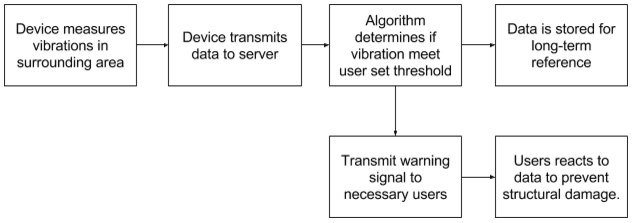
\includegraphics[width=0.85\textwidth]{functionmodel.png}
	\caption{High-level function model}
	\label{fig:Function Model}
\end{figure}
\subsection{Sub-Functions}
The above functions will be elaborated on to provide additional details.
\begin{enumerate}
	\item \textbf{Device measures vibrations in surrounding area}
	\begin{enumerate}
		\item The system is mounted to the surface to be monitored.
		\item Electrical energy is imported and stored in the system.
		\item Control Signals are imported into the system.
		\item System then measures vibrations.
	\end{enumerate}
	\item \textbf{Device transmits data to server}
	\begin{enumerate}
		\item Data is temporary logged then exported from the system.
		\item Data is received and stored long-term in the cloud.
	\end{enumerate}	
	\item \textbf{ Algorithm determines if vibration meets user set threshold}
	\begin{enumerate}
		\item User defined threshold is used to determine vibration severity.
		\item Vibrations above threshold are transmitted with high priority.
		\item Vibrations below threshold are stored for long-term reference.
	\end{enumerate}	
	\item \textbf{Data is stored for long term reference}
	\begin{enumerate}
		\item Data received is converted to electromagnetic energy and stored.
		\item User imports information into the system.
		\item System indicates data.
	\end{enumerate}	
	\item \textbf{Transmit warning to signal necessary users}
	\begin{enumerate}
		\item System receives signal from algorithm.
		\item System imports stored data.
		\item System exports data to users.
	\end{enumerate}	
	\item \textbf{Users reacts to data to prevent structural damage}
	\begin{enumerate}
		\item Human imports data from system.
		\item User responds to data.
	\end{enumerate}	
\end{enumerate}

\subsection{Refined Structure}
\begin{figure}[h!]
	\centering
	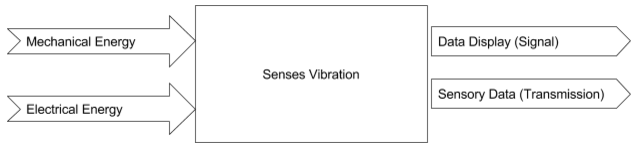
\includegraphics[width=0.85\textwidth]{refinedstructuremodel.png}
	\caption{Refined Structure Model}
	\label{fig:Refined Structure}
\end{figure}
\subsection{Function Decomposition Validation}
\begin{figure}[h!]
	\centering
	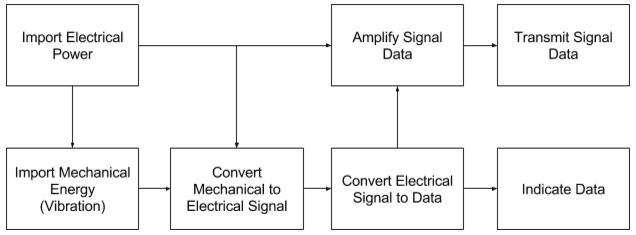
\includegraphics[width=0.85\textwidth]{decompmodel.png}
	\caption{Function Decomposition Model}
	\label{fig:Decomposition Model}
\end{figure}





\section{Competitive Benchmarking}

Comparable products exist for comparisons, Two companies utilizing vibration sensing for construction-related testing are Vibratech, and LORD Microsystems.  

The company Vibratech holds the gold-standard product for this type of testing with their Multi-Seis Plus model that has attachments for any type of vibrations created.  The Multi-seis plus models main parts, are a sensor box, attached to a transmitter box by way of an adjustable length cord.  Along with multiple ways to sense vibrations the Multi-Seis Plus also touts its ruggedness by being able to withstand all types of weather, being run over by a backhoe, and a pummeling from debris. It's limits include a short data transmission distance, and short battery life. The method of recharge for this device is a AC/DC power adapter that can be plugged into a wall outlet or generator.  

Lord Microsystems has a combination of devices, all of which utilize a central node transceiver that is communicating with multiple nodes placed around the construction site.  This device touts long battery life with its sensor node said to last about 18 months, but mentions nothing of battery life of the transceiver.  This type of transmitting from multiple nodes causes higher power drain from its central node, so extended duration would need to have minimal node placement. The transceiver also has Wi/Fi connection that can push to the web, which gives this device the edge on alerting at the moment.

\section{Competitive Improvements}

 Positive Resonance is aiming to find a way to improve upon the weaknesses observed with the current state of the art technologies. Our device needs to be as rugged as the Multi-Seis plus, have a battery life that exceeds the Multi-Seis plus, and is able to send data to the web, not only by Wi/Fi, but also 4G so that it can be completely self reliant. A solar recharging capability also will be added to allow longevity of batteries for projects monitoring for periods up to and over one month.\\
 
 Casing for the device needs to be resilient in all weather conditions and be rugged enough to be on a construction site. A product available for such tasks already could be a polycarbonate NEMA box.  This item is currently used in outdoor electrical applications for weather sensors. Functionality of this type of case comes from:
 
 
\begin{enumerate}
	\item Optional steel plating for further structural integrity and common grounding if needed.
	
	\item Mounting brackets for attachment to walls and other surfaces.
	
	\item Latches that secure the lid of the box, and a gasket to creating a waterproof seal.
		
	\item Casing easily allows ports for attachment of wires from the accelerometer and external solar panel.
	
		
\end{enumerate}	

To ensure casing will be able to withstand environmental conditions, testing will cover heat sensitivity, impact resilience, salt water and sand effects, \& water resistance.\\  

To do this we will test by:
\begin{enumerate}
	\item	Running the case through a cycle in the dishwasher.
	\item	Attaching the case to and ocean peer.
	\item   Prolonged sun exposure to test internal operating temperatures.   

	\end{enumerate}
	
Alternative protection will include:
\begin{enumerate}
	\item   Outlet attachments will be protected by silicone caps that will be created to prevent dirt and dust infiltration.
	\item   Shock absorption through addition of foam barriers within the case may be added to further protect sensitive internal components.\\
\end{enumerate}


For the programming of the 4G transceiver two tasks need to be completed and tested:
\begin{enumerate}
	\item 	Develop a server location that intakes signal information and deciphers it.  \\This server programming will need to:
	
	\begin{enumerate}
		\item Create waveform from incoming signal
		\item Analyze averages, highs, and lows.
		\item Recognize alerting ranges
		\begin{enumerate}
			\item From this server needs to pass information by text and email to client and cause device on location to alert with flashing LED.
		\end{enumerate}
		\item Allow user interfacing with device.
		\begin{enumerate}
			\item User should be able to request stored data from device.
			\item Possible device activation and de-activation
			\item Alert reset, or level adjustment.
		\end{enumerate}
		
		
	\end{enumerate}
	\item Develop a program that will take in signals from a sensor and push to a server.  \\This program will need to:
	\begin{enumerate}
		\item Communicate to and from server.
		\item Keep time and date.
		\item Receive sensor data.
		\item Store sensor data.
		\begin{enumerate}
			\item Time/date files
		\end{enumerate}
		\item Have its own alerting ranges in case device is not communicating with server.  
		\begin{enumerate}
			\item Mostly for LED activation.
			\item Needs to be overridden by server.
		\end{enumerate}
	\end{enumerate}
\end{enumerate}

To test the programming the following two tasks are needed:
\begin{enumerate}
\item  A number generator will be added to the program where values can be input either as normal values, abnormal, or at both.  The program will need to recognize given values and produce a waveform from values.  Once it does this, the alerting values need to be tested to make device recognize values.  Once this is shown to work, an alerting program will send a text response to the testers phone.  Then the email alert will be added and tested.  Lastly communication with actual device will be initiated and tested.

\item Initial programming will be created for receiving sensor data, and tracking time and date data for retrieval purposes.  Then internal alerting will be added and tested from incoming sensor values, looking for LED activation.  When these are working then connection to server will be assessed and responses will be tested based on given values to activate alerting through server.  \\
\end{enumerate}

For the power source our development process will go as follows:

\begin{enumerate}
	\item Evaluate long-life rechargeable batteries.
	\item Estimate power needs per electronic component and total power draw and choose battery voltage based on need.
	\item After building system.
	\begin{enumerate}
		\item 	Measure starting voltage, power device and re-measure voltage after 2 hours.
		\begin{enumerate}
			\item Determine average standing power draw from system.
		\end{enumerate}
		\item Recharge battery, measure voltage again then assess voltage used by device as it is sensing and sending for 2 hours.
		\begin{enumerate}
			\item Determine average working power draw from the system.
		\end{enumerate}
		\item Average power draw and calculate battery life before need of recharge.  
	\end{enumerate}
	\item Adjust Solar intake assist in battery life maintenance.
	
\end{enumerate}


\section{Engineering Specifications}
Engineering Specifications are attached to this document

\section{House of Quality}
The House of Quality is attached to this document.

\subsection{Summary}
The House of Quality is a useful tool that contains a great deal of information regarding the customer’s needs and the products functions.  The columns represent the products functions (How our product can be changed to meet the customer’s needs). The rows represent the customer’s needs (What objectives does the customer need the device to meet).  The customer needs are weighted according to what they believe are the most important.  The central grid shows the relationship between customer needs and product functions.  The values on the grid are weighted according to customer needs, and added together.  The final score shows how the different functions impact the customer needs.  In our House of Quality, it shows that the battery is the most important function in regards to the customer needs followed closely by the type of communication device.\\  \\
The triangle on top of the house shows how the different functions are related in the form of positive (improving one improves the other) and negative (improving one harms the other). For example, a negative relationship would be that improving the communication device would increase the drain on the battery, lowering the battery’s charge life.  The positive and negative symbols are placed at the intersection between the 2 diagonal rows for the functions.
The far right grid shows a comparison between how are device would meet our customers’ needs compared to our competitors.  Since this device is being made to meet our customers needs, our product surpasses our competitors in almost every area.


\section{Concept Generation}

\subsection{Concept 1}
\begin{figure}[ht!]
	\centering
	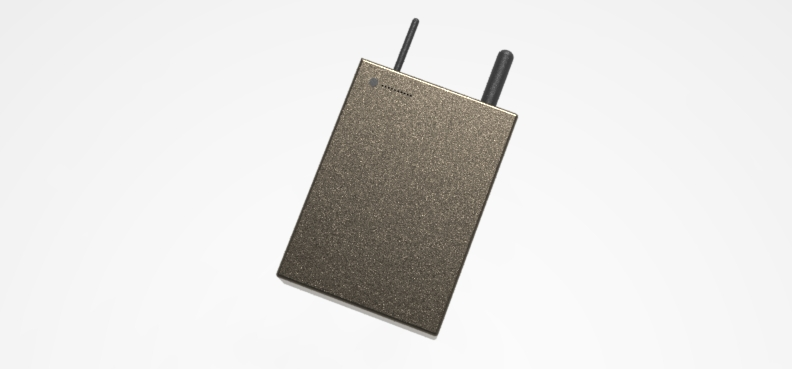
\includegraphics[width=1\textwidth]{model1.jpg}
	\caption{Concept 1}
	\label{fig:concept1}
\end{figure}
Concept one focuses on an all in one system. In this system once the device in mounted to a surface it will complete all necessary tasks including data collection, analysis and distribution.
Some advantages of this style of system include increased simplicity, sturdiness, and ease of relocation.
Disadvantages of a system such as this is space, battery capacity, signal interference, and vibration dampening.

\subsection{Concept 2}
\begin{figure}[ht!]
	\centering
	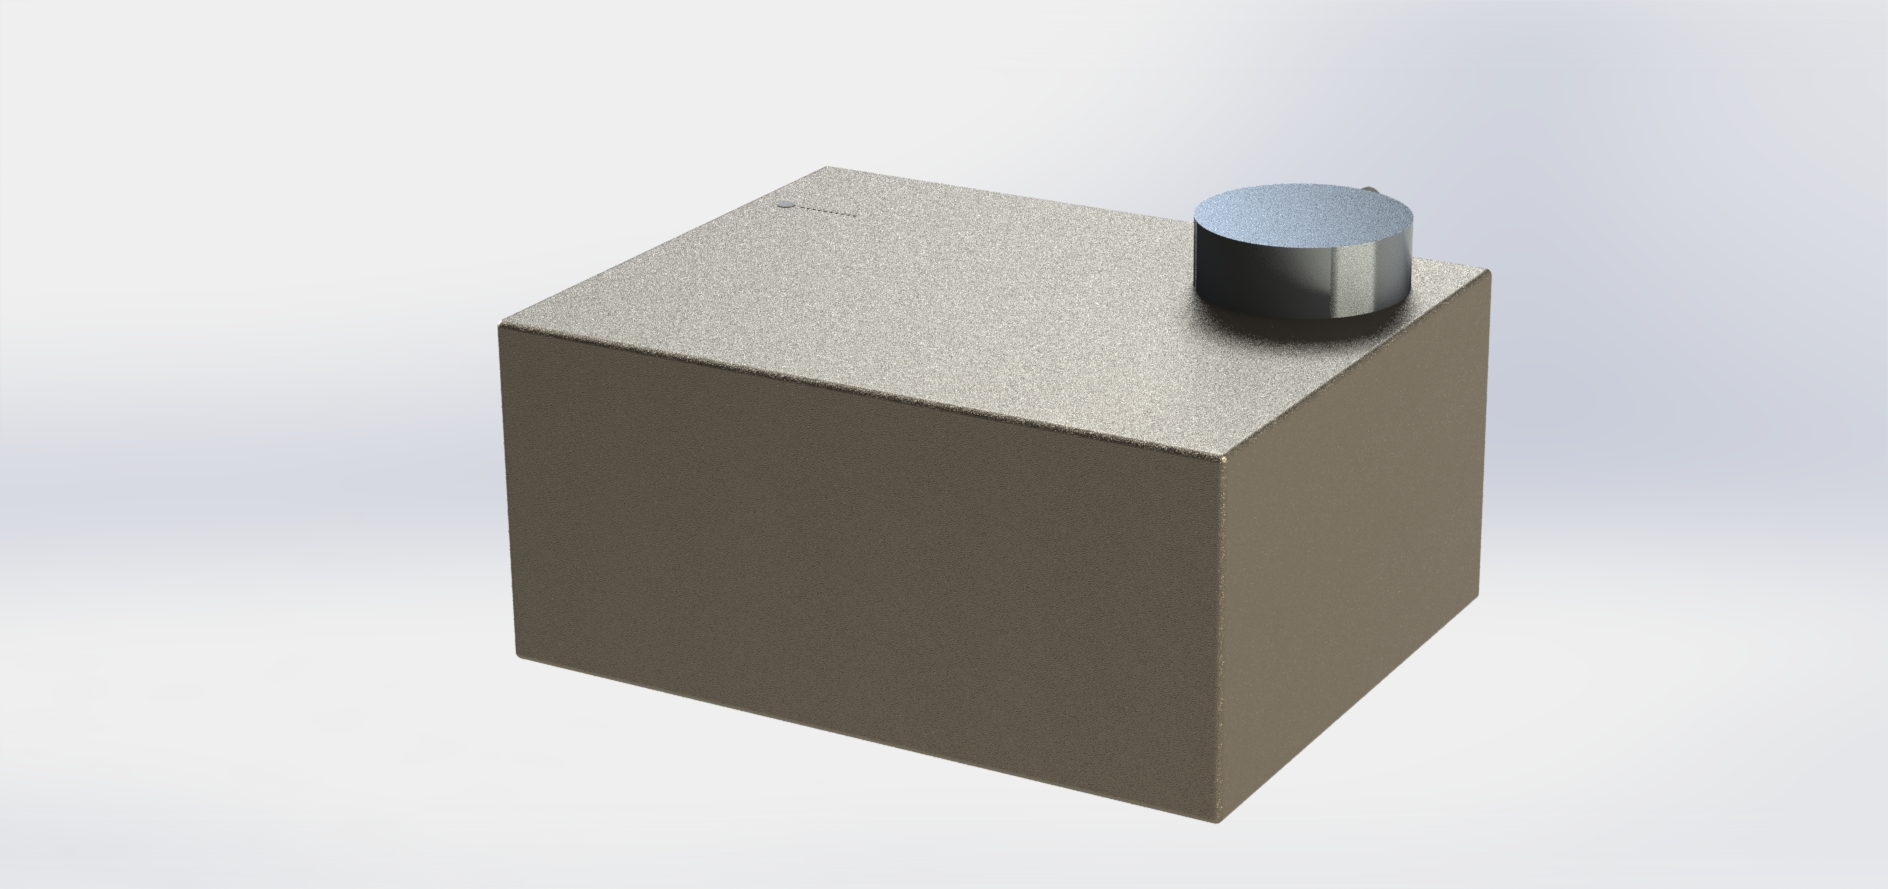
\includegraphics[width=1\textwidth]{model2.jpg}
	\caption{Concept 2}
	\label{fig:concept2}
\end{figure}
Concept two focuses on a main housing with a sensor that is separate from the body. In a system like this the sensor will be easily mountable to various surfaces, while the main housing will rest on the ground. The main housing will provide the battery, transceiver, analysis, and storage of the sensor. This system design allows for a larger space for extra battery power, and gives more opportunities for better sensor placement due to smaller sensor footprint.

\newpage

\section{Concept Selection}

\subsection{Refined Decision Matrix}
The refined decision matrix is attached to this document

\subsection{Technical Summary}
After completing the decision matrix, we were able to identify viable options and methods to complete the project while meeting the customer's requirements. After ranking each design component, respective to each characteristic of the project, we were able to refine our decision matrix based on a calculated score. The scores were generated by utilizing an assigned weight that was attributed to each customer requirement according to the level of urgency expressed by the customer. Afterwards, each individual design component was ranked on its inherent effectiveness towards supporting the customer requirements. In an effort to use the most appropriate design concept, the different scores were summed and analyzed. To refine the decision matrix the top concepts for each respective characteristic were chosen. If we observe our decision matrix we can see that for each design concept the concept designs with the highest score indicate that customer needs and functional requirements are covered. With communication, two options populate the section because in order to provide both 4G connectivity and WiFi connectability at a reasonable price separate components have to be implemented. We are confident that using a triple-axis accelerometer, Zigbee module, MG2639 4G module, Rechargeable Lithium Ion Battery, solar panel, and a Polycarbonate Nema Case we will be able to design and construct a wireless sensor module that will meet the customer's desired specifications. 

\section{Moving Forward}

Moving forward, our team plans to further refine our concepts, plan our testing, and create the validations plan. The refinement of our concept will consist of the continuation of past art and state of the art research, documenting the components  listed in the refined decision matrix, revisiting the functional model to determine if improvements can be made to create the best product possible. Our test will be designed with the customers requirements in mind. Thus, to guarantee their functional requirements our designs will be set to pass slightly stricter standards for dependability, robustness, and battery discharge cycle. In an effort to validate our project, our team plans to have more meetings with our customer to increase our understanding on what they want and require in order to guarantee a functional, reliable, and robust vibration sensing unit. 

\end{document}